\documentclass[11pt]{article}

\usepackage[T1]{fontenc}
\usepackage[utf8]{inputenc}
\usepackage[margin=1in]{geometry}
\usepackage{microtype}
\usepackage{amsmath,amssymb,booktabs,longtable,array,graphicx,xcolor}
\usepackage{natbib}
\usepackage[hidelinks]{hyperref}
\setlength{\emergencystretch}{2em}
\renewcommand{\topfraction}{0.92}
\renewcommand{\bottomfraction}{0.85}
\renewcommand{\textfraction}{0.06}
\renewcommand{\floatpagefraction}{0.75}

\newcommand{\pin}{p_{\mathrm{in}}}
\newcommand{\pout}{p_{\mathrm{out}}}
\newcommand{\deltap}{\Delta p}
\newcommand{\phys}{\mathrm{C}}
\newcommand{\raw}{\mathrm{Raw}}
\newcommand{\learned}{\mathrm{Learned}}
\newcommand{\simple}{\mathrm{Simple}}

\renewcommand{\thesection}{S\arabic{section}}
\title{Supplementary material:\\Earlier comparisons, sensitivity and provenance}
\author{Companion to the prescribed target-centering study}
\date{}
\begin{document}
\maketitle

This supplement separates descriptive source-validation, post-hoc optimizer
sensitivity, earlier A/B comparisons and historical erroneous-center evidence
from the fresh C/D primary results. Earlier numeric records are retained;
their prior-use, overlap and provenance limits remain applicable. Figure labels
that originally say ``Physics'' in the historical section refer to the erroneous
center H, not CorrectedPhysics. For reference, the original-unit log density is
\begin{equation}
\log p(Y\mid X)=\log q_\theta((Y-c(X)-\mu)/s\mid h(X))
 -\log s-\log F_\theta((\pin-c(X)-\mu)/s\mid h(X)).
\label{eq:likelihood}
\end{equation}

\section{Selected validation and optimizer sensitivity}
The source-validation scores selected checkpoints and are descriptive.
The optimizer-sensitivity analysis was added after C/D evaluation; it does
not change the frozen primary analysis. The same five trained models are
evaluated on C and D, so catalog repetitions are not additional seeds.
\begin{table}[!htbp]
\centering
\small
\setlength{\tabcolsep}{3pt}
\caption{All 16 prespecified contrasts on the source validation set ($N=100,042$ eligible events). These selected-checkpoint scores are descriptive; no fresh-event confidence interval is assigned. All quantities are in nats per eligible event. $\Delta$ is Raw-minus-Corrected NLL, averaged over five paired optimizer seeds; gain differences are more-information minus less-information. Seed SD is the sample SD across those five seeds, not a confidence interval or variation across independent datasets. $n_+$ counts positive seeds out of 5; zeros are not counted. Minimum and maximum retain adverse seed directions.}
\label{tab:information-source16}
\begin{tabular}{llrrrrr}
\toprule
Contrast & Train & Mean & Seed SD & Minimum & Maximum & $n_+/5$ \\
\midrule
$\Delta_{\mathrm{Hidden5}}$ & 10\% & $+0.005816$ & $0.000753$ & $+0.004758$ & $+0.006637$ & 5/5 \\
$\Delta_{\mathrm{Coarse2}}$ & 10\% & $+0.010700$ & $0.001138$ & $+0.009150$ & $+0.012058$ & 5/5 \\
$\Delta_{\mathrm{Coarse8}}$ & 10\% & $+0.003423$ & $0.001628$ & $+0.001031$ & $+0.005143$ & 5/5 \\
$\Delta_{\mathrm{Full5}}$ & 10\% & $+0.001999$ & $0.001677$ & $-0.000158$ & $+0.003785$ & 4/5 \\
\midrule
$\Delta_{\mathrm{Hidden5}}$ & 100\% & $+0.006126$ & $0.001026$ & $+0.005257$ & $+0.007301$ & 5/5 \\
$\Delta_{\mathrm{Coarse2}}$ & 100\% & $+0.010979$ & $0.001078$ & $+0.010059$ & $+0.012673$ & 5/5 \\
$\Delta_{\mathrm{Coarse8}}$ & 100\% & $+0.003296$ & $0.001165$ & $+0.002283$ & $+0.005261$ & 5/5 \\
$\Delta_{\mathrm{Full5}}$ & 100\% & $+0.001653$ & $0.001033$ & $+0.000289$ & $+0.003201$ & 5/5 \\
\midrule
$\Delta_{\mathrm{Coarse2}}-\Delta_{\mathrm{Hidden5}}$ & 10\% & $+0.004884$ & $0.000940$ & $+0.003738$ & $+0.005976$ & 5/5 \\
$\Delta_{\mathrm{Coarse8}}-\Delta_{\mathrm{Coarse2}}$ & 10\% & $-0.007277$ & $0.002145$ & $-0.009249$ & $-0.004007$ & 0/5 \\
$\Delta_{\mathrm{Full5}}-\Delta_{\mathrm{Coarse8}}$ & 10\% & $-0.001425$ & $0.002060$ & $-0.004455$ & $+0.000976$ & 1/5 \\
$\Delta_{\mathrm{Full5}}-\Delta_{\mathrm{Hidden5}}$ & 10\% & $-0.003817$ & $0.001589$ & $-0.006407$ & $-0.002297$ & 0/5 \\
\midrule
$\Delta_{\mathrm{Coarse2}}-\Delta_{\mathrm{Hidden5}}$ & 100\% & $+0.004854$ & $0.000626$ & $+0.004059$ & $+0.005597$ & 5/5 \\
$\Delta_{\mathrm{Coarse8}}-\Delta_{\mathrm{Coarse2}}$ & 100\% & $-0.007683$ & $0.000268$ & $-0.008089$ & $-0.007412$ & 0/5 \\
$\Delta_{\mathrm{Full5}}-\Delta_{\mathrm{Coarse8}}$ & 100\% & $-0.001643$ & $0.000861$ & $-0.002870$ & $-0.000732$ & 0/5 \\
$\Delta_{\mathrm{Full5}}-\Delta_{\mathrm{Hidden5}}$ & 100\% & $-0.004473$ & $0.001367$ & $-0.006900$ & $-0.003643$ & 0/5 \\
\bottomrule
\end{tabular}
\end{table}

\clearpage
% Generated post-hoc to known C/D outcomes. Do not edit numerical cells.
% Requires booktabs and longtable. Numeric effects are shown x 10^-3 nat/eligible event.
\begingroup
\scriptsize
\setlength{\tabcolsep}{2.5pt}
\begin{longtable}{llrrrrl}
\caption{Post-hoc paired optimizer-seed sensitivity on catalog C. All values except signs/fractions are in $10^{-3}$ nat per eligible event. $H,C2,C8,F$ denote Hidden5, Coarse2, Coarse8 and Full5. Signs list positive/negative/zero counts among five seeds. Each leave-one-out (LOO) mean averages the remaining four seeds; its range is not a confidence interval. C and D use the same five trained-seed pairs and are not pooled.}\label{tab:seed_sensitivity_C}\\
\toprule Contrast & Train (\%) & Mean (SD) & Seed range & $+/ - /0$ & LOO mean range & LOO sign\\ \midrule \endfirsthead
\toprule Contrast & Train (\%) & Mean (SD) & Seed range & $+/ - /0$ & LOO mean range & LOO sign\\ \midrule \endhead
$G_{H}$ & 10 & 6.272 (0.811) & [5.091, 7.058] & 5/0/0 & [6.075, 6.567] & positive\\
$G_{C2}$ & 10 & 10.399 (1.099) & [8.722, 11.643] & 5/0/0 & [10.088, 10.818] & positive\\
$G_{C8}$ & 10 & 3.082 (1.596) & [0.821, 4.583] & 5/0/0 & [2.707, 3.647] & positive\\
$G_{F}$ & 10 & 1.845 (1.855) & [-0.619, 3.899] & 4/1/0 & [1.331, 2.461] & positive\\
$G_{H}$ & 100 & 6.233 (1.125) & [5.069, 7.679] & 5/0/0 & [5.871, 6.524] & positive\\
$G_{C2}$ & 100 & 10.895 (1.060) & [9.564, 12.443] & 5/0/0 & [10.507, 11.227] & positive\\
$G_{C8}$ & 100 & 2.987 (1.211) & [1.978, 5.000] & 5/0/0 & [2.484, 3.239] & positive\\
$G_{F}$ & 100 & 1.550 (0.923) & [0.491, 2.979] & 5/0/0 & [1.192, 1.814] & positive\\
$G_{C2}-G_{H}$ & 10 & 4.127 (0.767) & [3.262, 5.019] & 5/0/0 & [3.905, 4.344] & positive\\
$G_{C8}-G_{C2}$ & 10 & -7.317 (2.210) & [-9.390, -4.184] & 0/5/0 & [-8.100, -6.799] & negative\\
$G_{F}-G_{C8}$ & 10 & -1.237 (2.137) & [-3.999, 1.645] & 1/4/0 & [-1.958, -0.547] & negative\\
$G_{F}-G_{H}$ & 10 & -4.427 (1.796) & [-7.407, -2.726] & 0/5/0 & [-4.852, -3.682] & negative\\
$G_{C2}-G_{H}$ & 100 & 4.662 (0.809) & [3.758, 5.809] & 5/0/0 & [4.375, 4.888] & positive\\
$G_{C8}-G_{C2}$ & 100 & -7.908 (0.441) & [-8.474, -7.443] & 0/5/0 & [-8.024, -7.766] & negative\\
$G_{F}-G_{C8}$ & 100 & -1.437 (0.673) & [-2.218, -0.632] & 0/5/0 & [-1.639, -1.242] & negative\\
$G_{F}-G_{H}$ & 100 & -4.683 (1.226) & [-6.658, -3.297] & 0/5/0 & [-5.030, -4.190] & negative\\
\bottomrule
\end{longtable}
\endgroup

\begingroup
\scriptsize
\setlength{\tabcolsep}{2.5pt}
\begin{longtable}{llrrrrl}
\caption{Post-hoc paired optimizer-seed sensitivity on catalog D. All values except signs/fractions are in $10^{-3}$ nat per eligible event. $H,C2,C8,F$ denote Hidden5, Coarse2, Coarse8 and Full5. Signs list positive/negative/zero counts among five seeds. Each leave-one-out (LOO) mean averages the remaining four seeds; its range is not a confidence interval. C and D use the same five trained-seed pairs and are not pooled.}\label{tab:seed_sensitivity_D}\\
\toprule Contrast & Train (\%) & Mean (SD) & Seed range & $+/ - /0$ & LOO mean range & LOO sign\\ \midrule \endfirsthead
\toprule Contrast & Train (\%) & Mean (SD) & Seed range & $+/ - /0$ & LOO mean range & LOO sign\\ \midrule \endhead
$G_{H}$ & 10 & 6.401 (0.778) & [5.344, 7.326] & 5/0/0 & [6.169, 6.665] & positive\\
$G_{C2}$ & 10 & 10.623 (1.277) & [8.786, 12.172] & 5/0/0 & [10.235, 11.082] & positive\\
$G_{C8}$ & 10 & 3.320 (1.609) & [0.878, 4.898] & 5/0/0 & [2.926, 3.931] & positive\\
$G_{F}$ & 10 & 1.876 (1.836) & [-0.491, 4.072] & 4/1/0 & [1.327, 2.467] & positive\\
$G_{H}$ & 100 & 6.543 (1.194) & [5.473, 7.943] & 5/0/0 & [6.193, 6.810] & positive\\
$G_{C2}$ & 100 & 11.196 (1.030) & [9.843, 12.587] & 5/0/0 & [10.848, 11.534] & positive\\
$G_{C8}$ & 100 & 3.332 (1.181) & [2.379, 5.241] & 5/0/0 & [2.855, 3.571] & positive\\
$G_{F}$ & 100 & 1.659 (0.973) & [0.371, 3.059] & 5/0/0 & [1.309, 1.981] & positive\\
$G_{C2}-G_{H}$ & 10 & 4.222 (1.046) & [3.301, 5.469] & 5/0/0 & [3.910, 4.452] & positive\\
$G_{C8}-G_{C2}$ & 10 & -7.302 (2.233) & [-9.356, -3.888] & 0/5/0 & [-8.156, -6.789] & negative\\
$G_{F}-G_{C8}$ & 10 & -1.445 (2.087) & [-4.331, 1.255] & 1/4/0 & [-2.120, -0.723] & negative\\
$G_{F}-G_{H}$ & 10 & -4.525 (1.713) & [-7.221, -2.631] & 0/5/0 & [-4.998, -3.851] & negative\\
$G_{C2}-G_{H}$ & 100 & 4.653 (0.837) & [3.790, 5.794] & 5/0/0 & [4.368, 4.869] & positive\\
$G_{C8}-G_{C2}$ & 100 & -7.864 (0.526) & [-8.549, -7.346] & 0/5/0 & [-7.993, -7.692] & negative\\
$G_{F}-G_{C8}$ & 100 & -1.673 (0.805) & [-2.704, -0.727] & 0/5/0 & [-1.909, -1.415] & negative\\
$G_{F}-G_{H}$ & 100 & -4.884 (1.447) & [-7.334, -3.581] & 0/5/0 & [-5.209, -4.271] & negative\\
\bottomrule
\end{longtable}
\endgroup

\clearpage
The following optional intervals describe the mean over optimizer seeds under
an approximate independent, normal seed-effect model conditional on the fixed
training data and evaluation catalog. They are post-hoc, pointwise and
unadjusted. With only five seeds they are sensitivity summaries, not a
confirmatory training-population analysis; C and D reuse the same seeds.
% Generated post-hoc to known C/D outcomes. Do not edit numerical cells.
% Requires booktabs and longtable. Numeric effects are shown x 10^-3 nat/eligible event.
\begingroup
\scriptsize
\setlength{\tabcolsep}{2.5pt}
\begin{longtable}{llrrl}
\caption{Optional exploratory Student-$t$ intervals on catalog C; not the default sensitivity table. With $n=5$, these nominal unadjusted 95\% intervals assume independent paired optimizer-seed draws and an approximately normal distribution of seed-level contrasts, conditional on the fixed training data, validation rule and evaluated catalog. They exclude training-dataset and simulator uncertainty, are not event-bootstrap intervals, and are not jointly calibrated over contrasts or C/D. Values are in $10^{-3}$ nat per eligible event.}\label{tab:seed_sensitivity_t_C}\\
\toprule Contrast & Train (\%) & Mean & Exploratory $t$ interval & Direction\\ \midrule \endfirsthead
\toprule Contrast & Train (\%) & Mean & Exploratory $t$ interval & Direction\\ \midrule \endhead
$G_{H}$ & 10 & 6.272 & [5.265, 7.278] & positive\\
$G_{C2}$ & 10 & 10.399 & [9.034, 11.764] & positive\\
$G_{C8}$ & 10 & 3.082 & [1.100, 5.064] & positive\\
$G_{F}$ & 10 & 1.845 & [-0.458, 4.148] & includes zero\\
$G_{H}$ & 100 & 6.233 & [4.836, 7.630] & positive\\
$G_{C2}$ & 100 & 10.895 & [9.579, 12.210] & positive\\
$G_{C8}$ & 100 & 2.987 & [1.483, 4.491] & positive\\
$G_{F}$ & 100 & 1.550 & [0.404, 2.695] & positive\\
$G_{C2}-G_{H}$ & 10 & 4.127 & [3.175, 5.080] & positive\\
$G_{C8}-G_{C2}$ & 10 & -7.317 & [-10.061, -4.573] & negative\\
$G_{F}-G_{C8}$ & 10 & -1.237 & [-3.890, 1.416] & includes zero\\
$G_{F}-G_{H}$ & 10 & -4.427 & [-6.656, -2.197] & negative\\
$G_{C2}-G_{H}$ & 100 & 4.662 & [3.657, 5.667] & positive\\
$G_{C8}-G_{C2}$ & 100 & -7.908 & [-8.456, -7.359] & negative\\
$G_{F}-G_{C8}$ & 100 & -1.437 & [-2.274, -0.601] & negative\\
$G_{F}-G_{H}$ & 100 & -4.683 & [-6.206, -3.160] & negative\\
\bottomrule
\end{longtable}
\endgroup

\begingroup
\scriptsize
\setlength{\tabcolsep}{2.5pt}
\begin{longtable}{llrrl}
\caption{Optional exploratory Student-$t$ intervals on catalog D; not the default sensitivity table. With $n=5$, these nominal unadjusted 95\% intervals assume independent paired optimizer-seed draws and an approximately normal distribution of seed-level contrasts, conditional on the fixed training data, validation rule and evaluated catalog. They exclude training-dataset and simulator uncertainty, are not event-bootstrap intervals, and are not jointly calibrated over contrasts or C/D. Values are in $10^{-3}$ nat per eligible event.}\label{tab:seed_sensitivity_t_D}\\
\toprule Contrast & Train (\%) & Mean & Exploratory $t$ interval & Direction\\ \midrule \endfirsthead
\toprule Contrast & Train (\%) & Mean & Exploratory $t$ interval & Direction\\ \midrule \endhead
$G_{H}$ & 10 & 6.401 & [5.435, 7.367] & positive\\
$G_{C2}$ & 10 & 10.623 & [9.037, 12.209] & positive\\
$G_{C8}$ & 10 & 3.320 & [1.322, 5.319] & positive\\
$G_{F}$ & 10 & 1.876 & [-0.403, 4.155] & includes zero\\
$G_{H}$ & 100 & 6.543 & [5.061, 8.025] & positive\\
$G_{C2}$ & 100 & 11.196 & [9.917, 12.475] & positive\\
$G_{C8}$ & 100 & 3.332 & [1.865, 4.799] & positive\\
$G_{F}$ & 100 & 1.659 & [0.451, 2.868] & positive\\
$G_{C2}-G_{H}$ & 10 & 4.222 & [2.923, 5.521] & positive\\
$G_{C8}-G_{C2}$ & 10 & -7.302 & [-10.075, -4.529] & negative\\
$G_{F}-G_{C8}$ & 10 & -1.445 & [-4.036, 1.147] & includes zero\\
$G_{F}-G_{H}$ & 10 & -4.525 & [-6.652, -2.398] & negative\\
$G_{C2}-G_{H}$ & 100 & 4.653 & [3.614, 5.692] & positive\\
$G_{C8}-G_{C2}$ & 100 & -7.864 & [-8.517, -7.211] & negative\\
$G_{F}-G_{C8}$ & 100 & -1.673 & [-2.673, -0.673] & negative\\
$G_{F}-G_{H}$ & 100 & -4.884 & [-6.680, -3.087] & negative\\
\bottomrule
\end{longtable}
\endgroup

\clearpage
\section{Numerical precision and support-boundary checks}
\label{sec:numerical_boundary}

The physical center and preprocessing calculations use NumPy float64. Targets,
centers, momentum, conditions and scales are then converted to torch.float32
for the learned density calculation. The optimizer and the validation mean
used for checkpoint selection are also float32. Saved per-event log scores are
promoted to float64 before paired subtraction, seed averaging, reported
reduction and bootstrap calculations. These stages must not be described as
float64 model inference. Selecting a different checkpoint using a float64
validation reduction would change the frozen training procedure.

The density uses stable log-sigmoid and softplus expressions. In base-flow
coordinates $a$ and $b$ for an event and its upper support bound, the truncated
log-survival expression is
\begin{equation}
 \log S=-\operatorname{softplus}(a)+\log[-\operatorname{expm1}(a-b)].
\end{equation}
This avoids directly subtracting two CDFs close to one. At the exact upper
boundary, log density and log survival are $-\infty$ and log CDF is zero.
The scorer rejects nonfinite density/decomposition values; legitimate
infinite log-tail probabilities are handled separately.

Three existing mathematical regression tests passed. Additional deterministic
checks used 18 tail cases per dtype, base support bounds from $-1000$ to
$1000$, and distances including one representable ULP below the boundary.
An untrained fixed flow in its identity tails was compared with a 100-digit
Decimal reference. In these synthetic checks, no events were generated or read, and no saved checkpoint was
evaluated, and no training was performed. Maximum observed absolute errors
were:
\begin{center}
\begin{tabular}{lrrrr}
\toprule
Dtype & Log density & Log CDF & Log survival & $|\mathrm{CDF}+\mathrm{SF}-1|$\\
\midrule
float32 & $9.14\times10^{-9}$ & $1.30\times10^{-9}$ & $1.05\times10^{-5}$ & $0$\\
float64 & $2.58\times10^{-15}$ & $2.04\times10^{-9}$ & $7.11\times10^{-15}$ & $2.02\times10^{-9}$\\
\bottomrule
\end{tabular}
\end{center}
The float64 log-CDF discrepancy reflects the default softplus linear
approximation above its threshold of 20; it is not evidence of uniform
$10^{-12}$ accuracy. Tested boundary values and log-survival gradients were
correct and finite where required. These checks are not a worst-case error
bound over every learned spline parameterization or device.

Input resolution is a separate limit. At momentum 0.3, 0.65 and 1.0 GeV/$c$,
an input only one float64 ULP inside the upper support becomes equal to the
bound after float32 conversion. This establishes a rounding possibility.
The follow-up audit below measures its incidence in the complete formal C/D
samples without modifying those samples or rerunning the density models.

\subsection{Complete event coverage and input margins}

This follow-up audit was performed after the C/D results were known. All
500,000 launched ledger records in each catalog were read. Eligibility was
reconstructed from the saved first-visit entry/exit geometry and exit momentum,
without retracing Geant4 steps. The resulting 499,285 C and 499,275 D eligible
rows matched every saved scoring input, including event identifiers and their
order. The 715 and 725 ineligible events were excluded by the physical event
contract before scoring, not by numerical filtering. The saved target agreed
bitwise with the independently recomputed $Y=p_{\rm in}-p_{\rm out}$.

For each eligible row, define
\begin{equation}
 m_{32}=\operatorname{fl}_{32}\!\left(
 \operatorname{fl}_{32}(p_{\rm in})-\operatorname{fl}_{32}(Y)\right).
\end{equation}
Both catalogs have zero nonfinite, zero and negative margins. None has a
positive margin at or below $10^{-3}$ GeV/$c$, or at or below 1024 downward
ULPs at $p_{\rm in}^{(32)}$; the smallest margin-to-ULP ratios are
$8.2840175\times10^6$ and $8.311172\times10^6$, respectively. The cumulative
thresholds were fixed before the ledger scan. Here one downward ULP is
$p^{(32)}-\operatorname{nextafter}(p^{(32)},-\infty)$.
Table~\ref{tab:actual_support_margins} reports the distribution after computing
the subtraction in float32 and promoting its result to float64 for linear
quantile interpolation. A float64 difference of two rounded inputs is a
distinct diagnostic, retained separately in the audit records.

\begin{table}[!htbp]
\centering\small
\setlength{\tabcolsep}{4pt}
\caption{Actual float32 support-margin distributions, in GeV/$c$. Counts
include all eligible events. Zero, negative and nonfinite counts are zero in
both catalogs. The complete finer quantiles and seven momentum-bin summaries
are retained with the aggregate audit.}
\label{tab:actual_support_margins}
\begin{tabular}{lrrrrrr}
\toprule
Catalog & Events & Minimum & 1\% & Median & 99\% & Maximum\\
\midrule
C & 499,285 & 0.295779943 & 0.306910386 & 0.649518907 & 0.992840517 & 0.999970257\\
D & 499,275 & 0.297881365 & 0.306801179 & 0.650127709 & 0.992949682 & 0.999970496\\
\bottomrule
\end{tabular}
\end{table}

All 240 registered models per catalog retained the complete eligible-event
count and event-order digest. Recomputing only their frozen centers and
standardization, without evaluating a neural flow, reproduced all 960 saved
$z$ and $b$ arrays bitwise: 479,308,800 values, with no mismatch. The smallest
$b-z$ was 751.749807, and no saved $z$ reached or exceeded $b$.
All 5280 saved model-component arrays passed their recorded byte, shape and
dtype checks, and all event log densities were finite. Together these checks
show that no eligible row was silently dropped or numerically rejected from
the completed scores. They are a ledger and preprocessing reconciliation,
not a new neural-density evaluation or a validation of the transport physics.

\subsection{Actual support log-CDFs and their mathematical scale}

Across all 480 registered model--catalog evaluations, every saved support
log-CDF is float32 negative zero: 239,654,400 entries, zero nonzero values and
zero nonfinite values. Thus all its recorded quantiles are zero. These are
repeated model--event evaluations, not that many independent events; the 20
Full rerun pairs per catalog retain their exact duplicate identities.
Table~\ref{tab:actual_support_bounds} separates the primary 80 runs from the
160 earlier registered runs.

\begin{table}[!htbp]
\centering\small
\caption{Range of recorded standardized support bounds across every eligible
event and model in each cohort. Each model has bound 8 for both spline layers.
All support log-CDF entries are negative zero; all saved $z<b$.}
\label{tab:actual_support_bounds}
\begin{tabular}{llrrr}
\toprule
Catalog & Cohort & Model--event entries & Minimum $b$ & Maximum $b$\\
\midrule
C & Primary 80 & 39,942,800 & 761.355408 & 2776.529053\\
C & Earlier 160 & 79,885,600 & 761.350159 & 2776.529053\\
D & Primary 80 & 39,942,000 & 761.354797 & 2776.541260\\
D & Earlier 160 & 79,884,000 & 761.349548 & 2776.543945\\
\bottomrule
\end{tabular}
\end{table}

The zeros have a quantitative explanation. Every saved bound exceeds 761.349,
well outside the spline interval $[-8,8]$. Each layer is exactly the identity
there, so its transformed base bound equals $b$, independently of the neural
conditioner outputs. With the standard logistic base,
\begin{equation}
 \epsilon(b)=1-F_\theta(b\mid h)=\frac{1}{1+e^b},\qquad
 \eta(b)=-\log F_\theta(b\mid h)=\log(1+e^{-b}).
\end{equation}
For $b>0$, both satisfy $0<\epsilon(b),\eta(b)<e^{-b}$. The smallest recorded
bound therefore gives $\epsilon,\eta<10^{-330}$ for every evaluated entry.
The excluded probability mass and the likelihood normalization correction
are mathematically positive, but are smaller than half the smallest positive
float64 subnormal number. A float64 re-expression would also round them to
zero; it would not reveal a representable nonzero distribution. The aggregate
audit retains the $b$ quantiles and log-domain bounds, rather than assigning
artificial nonzero probabilities.

This certificate concerns the mathematical logistic function evaluated at the
saved rounded bounds. It uses the verified identity-tail construction and
does not rerun the neural networks in float64. It explains why normalization
has no observable contribution for these models and catalogs; the term remains
in the likelihood and is not assumed negligible for other models or inputs.


\section{Earlier corrected comparisons and reused A/B evaluations}
\label{app:earlier_corrected}

This appendix retains the earlier corrected-model results as a separate evidence
stage. Its Hidden conditioner has two inputs, whereas Hidden5 in the new primary
experiment has five input positions. A/B have disclosed prior use. The earlier
physical-group and location reviews were post hoc; their status is not changed
by the prespecified follow-up on fresh C/D. Numerical values below refer to the
earlier designs and datasets.

\subsection{Earlier matched protocols}


The common optimization protocol is Adam with learning rate $3\times10^{-4}$,
batch size 512, gradient-norm clipping at 5.0, zero weight decay and dropout,
validation at update 1 and every 500 updates,
and a 20,000-update upper limit. The checkpoint is the lowest source-validation
original-unit NLL within the fixed budget. Gradient-norm diagnostics, validation histories,
checkpoint states, and per-event likelihood components are retained.

The conditioner comparison contains 60 fits: Raw, H and CorrectedPhysics;
Full and Hidden; 10\% and 100\% training fractions; and five optimizer seeds
(3101--3105). All use Small width 32. Ordered training subsets and minibatch
random-number seeds match across representations and conditioners, with
initialization matched within each conditioner. The Full matrix comprises
Raw, Simple, Learned and CorrectedPhysics at widths 32 and 128, fractions
10\%, 30\% and 100\%, and the same five seeds. Its 120 fits include 20
eligible models from the conditioner comparison, giving 160 distinct fitted
models in total. Reused models are overlapping evidence.

All fitted centers and preprocessing use only the active training subset.
Both earlier designs use catalog 4101 and nested training subsets ordered by
the SHA256 hash of the catalog identifier and event UID.
Learned selects its penalty with three training-only folds defined by row
index modulo three after sorting the subset by its declared catalog/event
hash. The selected checkpoint minimizes source-validation original-unit NLL
within the fixed update budget. Selection uses the float32 validation mean;
reported means use float64 accumulation of saved per-event scores. All 160
models were subsequently scored on each of A and B, without refitting or
selection. Independent artifact and arithmetic checks are summarized in
Appendix~\ref{app:verification}.

The Full/Hidden comparison was the primary question in the earlier two-conditioner stage.
Capacity, training-fraction and fitted-center comparisons are secondary in the
paper's argument, while retaining their originally prespecified status within
their own experiment protocol. Physical-group and residual-location reviews
are exploratory, post-hoc analyses. H is an implementation-history control.
This presentation hierarchy does not revise the historical protocols or
retroactively make an exploratory analysis prespecified.

The prespecified conditioner comparisons are Raw minus CorrectedPhysics, Raw
minus H, H minus CorrectedPhysics, and their Full-minus-Hidden differences.
The Full matrix prespecifies Raw minus CorrectedPhysics, Learned minus
CorrectedPhysics and Simple minus Raw at every capacity/fraction, together
with three capacity and two fraction interactions of the Raw-minus-Corrected
gain. All contrasts are reported in nat/event, with positive
NLL(left)$-$NLL(right) favoring the right model. For the main representation
comparison, define
\begin{equation}
 \Delta_h=\mathrm{NLL}(\raw,h)-\mathrm{NLL}(\mathrm{C},h),\qquad
 \mathcal I=\Delta_{\rm Full}-\Delta_{\rm Hidden},
 \label{eq:earlier_contrast}
\end{equation}
where C denotes CorrectedPhysics. The interaction $\mathcal I$ compares relative gains,
not the two models' absolute likelihoods. Means, sample standard deviations
and all five paired seed values are retained. Seed spread describes optimizer
variation on shared data rather than uncertainty across independently sampled
datasets. Validation results are descriptive because validation selected
checkpoints. Holding updates fixed across fractions does not equalize epochs
or per-event optimization exposure.



\subsection{Earlier Full/Hidden comparison on A/B}
\label{sec:conditioner_results}

CorrectedPhysics improves mean NLL relative to Raw under both conditioners in
the matched Small-capacity comparison. On A, Full gains at 10\% and 100\%
are $+0.001799$ and $+0.001573$ nat/event, while Hidden gains are $+0.006720$
and $+0.007009$. On B, the corresponding Full gains are $+0.001728$ and
$+0.001412$, and Hidden gains are $+0.006372$ and $+0.006542$.
Every Hidden seed is positive in each block/fraction combination. Full at
10\% retains one negative seed on each block. Figure~\ref{fig:corrected_core_confirmation}
shows every seed alongside the selected-validation results in
Table~\ref{tab:corrected_core}.

\begin{table}[t]
\centering
\caption{Small-capacity source-validation contrasts in nat/event.
SD is the sample SD across five paired optimizer seeds sharing source data,
not an independent-data confidence interval. Full-minus-Hidden rows subtract
the two within-context contrasts, not the absolute NLLs.}
\label{tab:corrected_core}
\begin{tabular}{lrrrr}
\toprule
Comparison & Fraction & Mean & Seed SD & Direction \\
\midrule
Full & 10\% & $+0.001999$ & $0.001677$ & 4/5 positive \\
Full & 100\% & $+0.001653$ & $0.001033$ & 5/5 positive \\
Hidden & 10\% & $+0.006399$ & $0.000652$ & 5/5 positive \\
Hidden & 100\% & $+0.006720$ & $0.001430$ & 5/5 positive \\
Full minus Hidden & 10\% & $-0.004400$ & $0.001994$ & 5/5 negative \\
Full minus Hidden & 100\% & $-0.005067$ & $0.001039$ & 5/5 negative \\
\bottomrule
\end{tabular}
\end{table}

The gain is larger in Hidden: the Full-minus-Hidden interactions $\mathcal I$ are
$-0.004921$ and $-0.005436$ nat/event on A, and $-0.004645$ and $-0.005130$
on B, at 10\% and 100\%, respectively. Every paired seed has this direction.
This conditioner dependence is a comparison of gains against the Raw baseline
within each context. Corrected Hidden still has higher absolute NLL than
Corrected Full, by $0.019643$ and $0.019721$ nat/event on A, and $0.018815$
and $0.018891$ on B. Source validation has the same relative and absolute
directions, with Hidden-minus-Full absolute differences of $0.019321$ and
$0.019318$ nat/event. These findings apply to the two tested fractions at
Small capacity.

\begin{figure}[t]
\centering
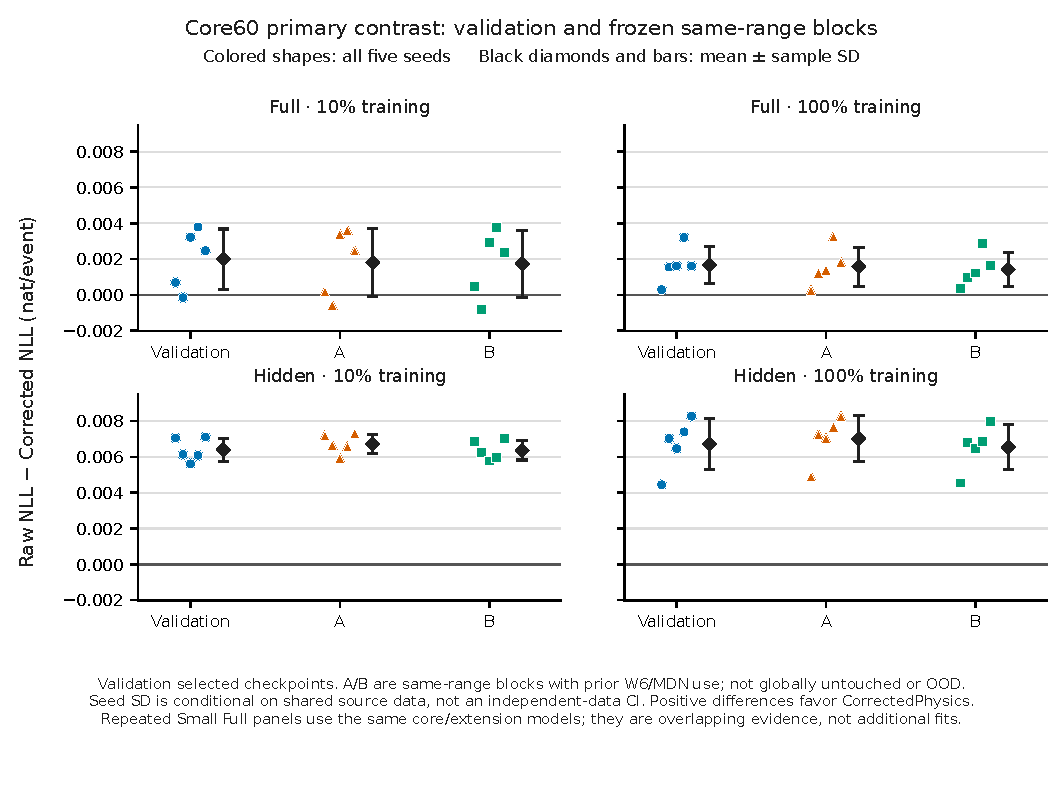
\includegraphics[width=\linewidth]{figures/correction_core_confirmation.pdf}
\caption{Core Raw-minus-Corrected contrasts on selected validation and frozen
A/B. All five seeds and sample SD are shown on one shared scale. Hidden's
larger overall mean gain does not imply better absolute NLL or improvement in
every conditional group. A/B retain legacy same-range provenance.}
\label{fig:corrected_core_confirmation}
\end{figure}

\subsection{Secondary comparisons: capacity, training fraction and fitted centers}
\label{sec:corrected_full_confirmation}

The expanded Full matrix places the physical center alongside two fitted
centers and varies model capacity and training fraction.
CorrectedPhysics has lower mean NLL than Raw in all six capacity/fraction
groups on A and separately on B. The gains range from $0.001341$ to
$0.002326$ nat/event on A and from $0.001231$ to $0.002265$ on B
(Figure~\ref{fig:corrected_full_confirmation}). The selected-validation range
is $0.001616$--$0.002393$ nat/event. The Small 10\% comparison includes one
negative seed on all three datasets; Small 30\% includes an additional
negative seed on A. These exceptions remain in the complete tables.

All six Learned-minus-Corrected mean contrasts are also positive on validation,
A and B. Conversely, all six Simple-minus-Raw mean contrasts are negative:
the simple fitted center improves on Raw in mean, so mean improvement over Raw
is not unique to the physical center. Individual seed exceptions include
Learned-minus-Corrected at Large 100\% on all three datasets and at Small
30\% on A. Appendix Table~\ref{tab:full-primary-complete} and the complete A/B
tables retain all prespecified contrasts rather than only favorable means.

\begin{figure}[t]
\centering
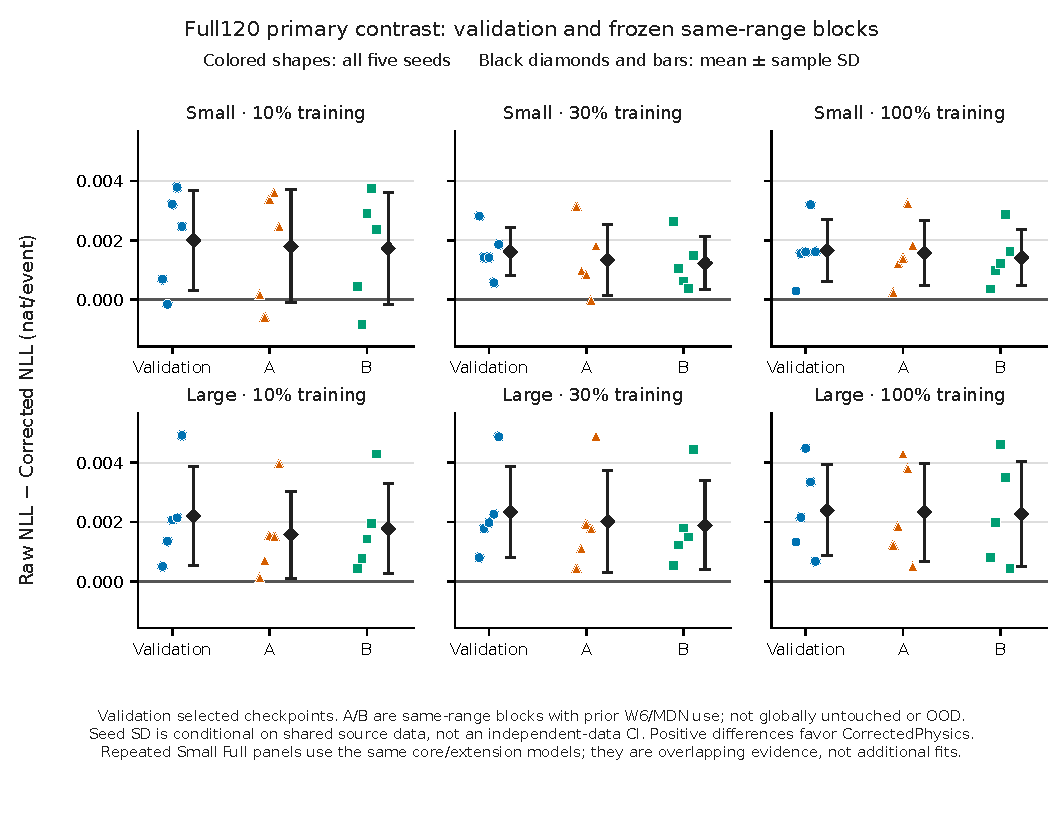
\includegraphics[width=\linewidth]{figures/correction_full_confirmation.pdf}
\caption{Full-conditioner Raw-minus-Corrected comparison at both capacities and
all three fractions. Negative seeds are retained. The Small Full 10\%/100\%
models overlap with the core figure and are not additional replications.
All other prespecified comparisons remain in the complete A/B tables.}
\label{fig:corrected_full_confirmation}
\end{figure}

Capacity and fraction effects are less consistent than the mean direction of
the representation comparison. The Small-minus-Large interaction of
Raw-minus-Corrected gains at 10\% changes mean sign between validation and A,
and is slightly negative on B. Fraction interactions also have mixed seed
directions. These results do not establish a monotonic capacity or sample-size
relationship under the fixed-update budget. An additional post-hoc comparison
of absolute NLL finds Small-minus-Large means below zero in all 36
representation/fraction/dataset groups. Thus a larger relative representation
gain at Large capacity does not identify the better absolute predictor in
this experiment.

\subsection{Post-hoc conditional performance: mean gains coexist with local losses}
\label{sec:local_results}

The 42 momentum--thickness--charge groups were fixed before scoring, but this
review of their heterogeneity was added after inspecting completed results.
It is descriptive and post-hoc. For each Hidden fraction on each block,
18 group means favor CorrectedPhysics and 24 favor Raw. The negative-mean
groups contain about 57.14\% of events; this is the event share of those bins,
not the fraction of individual events with worse likelihood. They occupy
momenta $[0.4,0.6)$ and $[0.8,1.0]$ GeV/$c$ across every thickness and charge.
The large event-weighted gain in $[0.3,0.4)$, about $0.086$--$0.094$ nat/event,
dominates the positive overall mean. Group means span approximately
$-0.048$ to $+0.123$ nat/event, and 12--13 groups have all five seed contrasts
negative. These observed bin means qualify the overall Hidden benefit. They do not,
by their count alone, establish a population-level regional failure pattern
or a significance claim. Conditional calibration is a separate property.

Each Full condition also has 2--9 negative group means, although none is negative
for every seed. All thickness-marginal means are positive, showing how a coarse
marginal can conceal momentum heterogeneity. These group counts are not
independent successful trials, and group means do not resolve within-bin behavior.

Table~\ref{tab:local_hidden} places the overall Hidden means alongside the
local contrast ranges. The repeated sign pattern across blocks and fractions
is a descriptive feature of these fixed bins, not an independent-bin test.

\begin{table}[t]
\centering
\caption{Post-hoc Hidden group summaries at Small capacity, in nat/event. A positive overall
Raw-minus-Corrected mean coexists with negative means in 24 of the 42
predefined groups. Ranges are across five-seed group means, not across events.
The last column counts groups in which all five seed contrasts are negative.}
\label{tab:local_hidden}
\small
\setlength{\tabcolsep}{4pt}
\begin{tabular}{llrrrr}
\toprule
Block & Fraction & \shortstack{Overall\\mean} & \shortstack{Negative\\groups} & Group mean range & \shortstack{All-five\\negative} \\
\midrule
A & 10\% & $+0.006720$ & 24/42 & $[-0.047278,+0.123132]$ & 13 \\
A & 100\% & $+0.007009$ & 24/42 & $[-0.041985,+0.117412]$ & 12 \\
B & 10\% & $+0.006372$ & 24/42 & $[-0.047979,+0.119093]$ & 12 \\
B & 100\% & $+0.006542$ & 24/42 & $[-0.042919,+0.116428]$ & 13 \\
\bottomrule
\end{tabular}
\end{table}

\subsection{Post-hoc location diagnostic and the erroneous-center control}
\label{sec:location_results}

The earlier matched 60-run comparison includes H to distinguish the intended physical
center from the earlier unit-inconsistent implementation. Under the same
controlled protocol, the source-validation Hidden Raw-minus-H means are
$-0.087870$ and $-0.087728$ nat/event at 10\% and 100\%, with every seed
negative. On A/B, the Hidden deficit remains approximately $0.088$ nat/event.
The unit-consistent center has the opposite mean direction, as reported in
Section~\ref{sec:conditioner_results}. This control establishes that the old
deficit does not characterize CorrectedPhysics; it was introduced after the
implementation error was identified, rather than as a planned physical
alternative in the original study.

Every representation separately fits $\mu=\operatorname{mean}_{\rm train}(Y-c)$.
Adding a constant to $c$ changes $\mu$ by the opposite constant; the standardized
residual and support coordinate absorb that offset. The amplitude of $c$ alone therefore does not predict a likelihood gain;
its variation across conditions must be considered after this offset is absorbed.

After viewing the validation results, we examined momentum-bin residual means
within each retained condition $W=(t,q)$ on the source diagnostic split. For
seven momentum bins $j$, with count $n_{jW}$ and residual mean $m_{jW}$, define
\begin{equation}
 N_W=\sum_j n_{jW},\quad
 m_W=\frac{\sum_j n_{jW}m_{jW}}{N_W},\quad
 v_W=\frac{\sum_j n_{jW}(m_{jW}-m_W)^2}{N_W}.
\end{equation}
The pooled metric is $[\sum_W N_W v_W/\sum_W N_W]^{1/2}$.
It is $8.01561\times10^{-6}$, $1.40700\times10^{-5}$ and
$5.88169\times10^{-6}$ GeV/c for Raw, H and CorrectedPhysics, respectively.
Both fractions give the same original-unit centered metric because the global
training mean cancels. This is variation of bin means, not within-bin event
variance; no confidence interval is estimated.

The global 42-bin location measure also contains between-thickness/charge
variation. H lowers that global measure while increasing the within-$W$
momentum measure, so the global measure must not be used as a Hidden-specific
burden. CorrectedPhysics lowers the within-$W$ metric. This post-hoc pattern is
consistent with the NLL directions but does not identify their unique cause:
finite-bin averaging, conditional shape/scale, support and optimization may
also contribute. The pooled diagnostic does not explain which individual
groups gain or lose likelihood.

\begin{figure}[t]
\centering
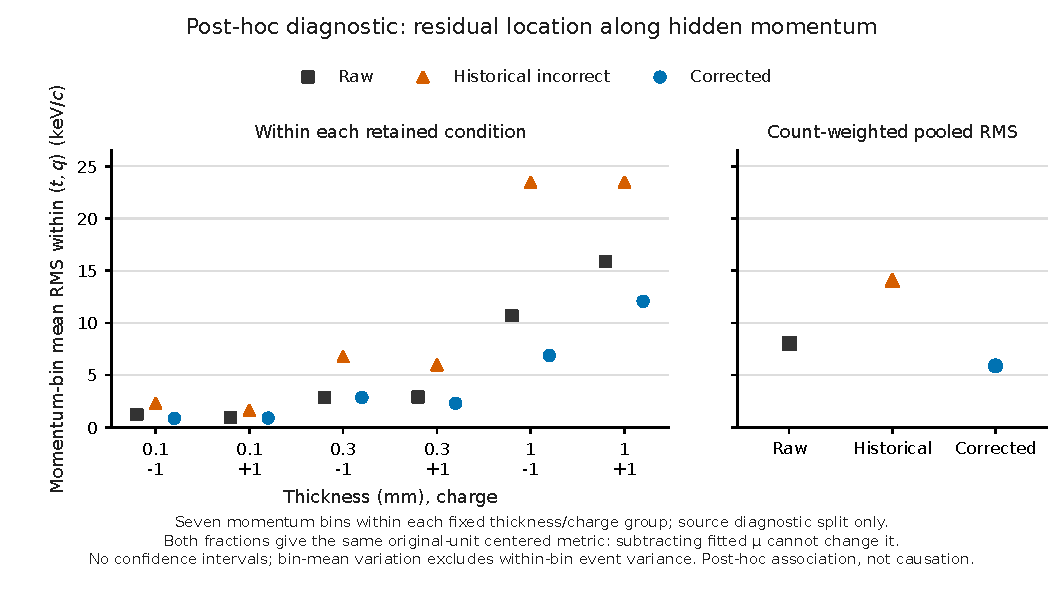
\includegraphics[width=0.95\linewidth]{figures/correction_within_condition.pdf}
\caption{Post-hoc residual-location diagnostic within fixed thickness and
charge. Every retained-condition group and the count-weighted pooled metric
are shown. Both fractions are retained in the source tables and coincide in
original units after centering. The plot contains no confidence intervals and
is neither a prespecified primary comparison nor causal identification.}
\label{fig:correction_location}
\end{figure}


\clearpage
\section{Verification and additional validation displays}
\label{app:verification}

The earlier corrected 60-model conditioner study and 120-entry Full matrix
use catalog 4101 across all representations, fractions and conditioners.
Independent checks cover every saved checkpoint,
source/protocol/data identity and paired event order. All source-validation
means were reconstructed from the 100,042 saved per-event scores. Every model
was replayed on 4,096 ordered validation events. The maximum absolute
log-density discrepancies were $1.04904\times10^{-5}$ for the 60-model
conditioner study and $1.383\times10^{-5}$ for the Full matrix, within the
declared replay tolerances. The reused models retain their original checkpoint,
preprocessing and event-order identities.

The frozen A/B evaluation covers 320 model/block scores for 160 unique models.
Independent saved-output verification checked all model identities, 410
prespecified seed contrasts, 82 five-seed summaries and grouped arithmetic.
It did not perform a second raw-event likelihood replay. Complete tables
follow; the selected-validation figures below retain all seeds, including
negative values, and the Full direct-comparison display is supplemented by
the five prespecified interaction groups in the tables.

\begin{figure}[!htbp]
\centering
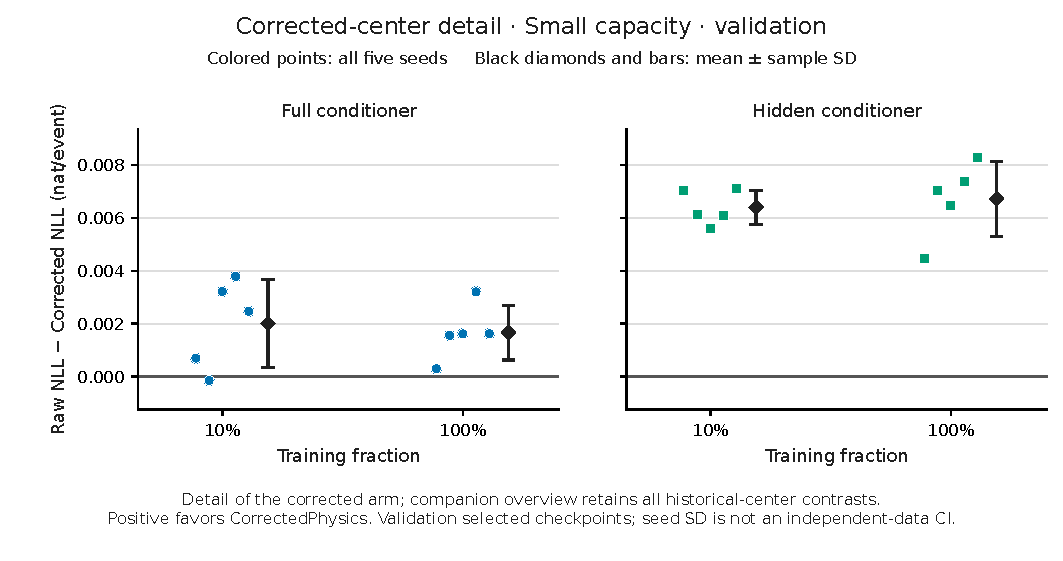
\includegraphics[width=0.95\linewidth]{figures/correction_core_detail.pdf}
\caption{All five corrected-arm seed contrasts and their mean with sample SD.
This detailed common scale retains the negative Full 10\% seed. The companion
complete overview in the repository includes the much larger erroneous-center
Hidden deficit; it is not discarded to produce this detail.}
\label{fig:corrected_core}
\end{figure}

\begin{figure}[!htbp]
\centering
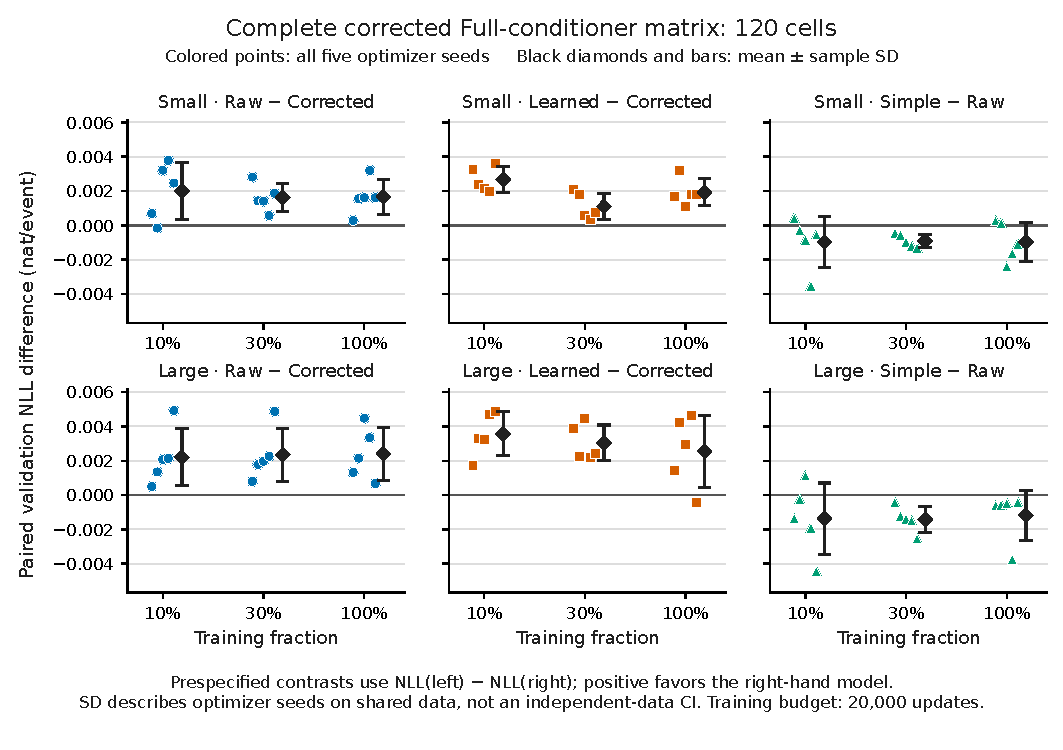
\includegraphics[width=\linewidth]{figures/correction_full_matrix.pdf}
\caption{Complete corrected Full matrix. Every displayed group retains all five
paired seed contrasts, with mean and sample SD. Positive NLL(left)$-$NLL(right)
favors the right model. The common scale includes negative seeds. Validation
selected checkpoints; these bars describe shared-data optimizer variation,
not independent-data confidence intervals.}
\label{fig:corrected_full_matrix}
\end{figure}

\clearpage
% Generated only from complete independently verified results. Requires longtable and booktabs.
\section{Complete corrected-study prespecified contrasts}
Differences are original-unit NLL(left)$-$NLL(right), in nat/event; positive favors the right model.
Every group retains five seeds. SD is sample SD conditional on shared data, not an independent-data confidence interval.
R: Raw; C: CorrectedPhysics; H: HistoricalIncorrectPhysics; L: Learned; S: Simple. Sm/Lg are Small/Large.
dCap denotes Small-minus-Large and dFrac denotes 10\%-minus-100\% differences of R-C.
In the A/B tables, Sm-Lg capacity rows and 10-100 fraction rows denote those same interaction contrasts.
Validation selected checkpoints. A/B are same-range blocks with prior W6/MDN use; they are not globally untouched or OOD.
The Small Full models shared between the core and extension are overlapping evidence.
\begingroup\scriptsize
\setlength{\tabcolsep}{3pt}
\begin{longtable}{lllrrrr}
\caption{All 23 Full120 validation primary groups. All five seeds retained; +/$-$/0 counts use unrounded values.}\label{tab:full-primary-complete}\\
\toprule
Capacity & Fraction & Contrast & Mean & SD & Range & +/$-$/0 \\
\midrule\endfirsthead
\toprule
Capacity & Fraction & Contrast & Mean & SD & Range & +/$-$/0 \\
\midrule\endhead
\bottomrule\endfoot
Sm & 10 & R-C & +0.001998758 & 0.001677306 & [-0.000158174, +0.003784627] & 4/1/0 \\
Sm & 10 & L-C & +0.002670894 & 0.000734112 & [+0.001957503, +0.003621019] & 5/0/0 \\
Sm & 10 & S-R & -0.000972340 & 0.001509722 & [-0.003540776, +0.000402922] & 1/4/0 \\
Lg & 10 & R-C & +0.002193965 & 0.001660770 & [+0.000499914, +0.004919161] & 5/0/0 \\
Lg & 10 & L-C & +0.003560944 & 0.001282595 & [+0.001702869, +0.004856525] & 5/0/0 \\
Lg & 10 & S-R & -0.001377730 & 0.002079980 & [-0.004457797, +0.001117632] & 1/4/0 \\
Sm & 30 & R-C & +0.001616113 & 0.000816585 & [+0.000568854, +0.002813414] & 5/0/0 \\
Sm & 30 & L-C & +0.001102159 & 0.000768607 & [+0.000343137, +0.002068916] & 5/0/0 \\
Sm & 30 & S-R & -0.000909031 & 0.000381837 & [-0.001322160, -0.000466012] & 0/5/0 \\
Lg & 30 & R-C & +0.002335295 & 0.001520685 & [+0.000795918, +0.004871455] & 5/0/0 \\
Lg & 30 & L-C & +0.003035869 & 0.001048371 & [+0.002214564, +0.004461310] & 5/0/0 \\
Lg & 30 & S-R & -0.001424522 & 0.000756559 & [-0.002547124, -0.000433972] & 0/5/0 \\
Sm & 100 & R-C & +0.001652905 & 0.001033412 & [+0.000288808, +0.003201191] & 5/0/0 \\
Sm & 100 & L-C & +0.001920352 & 0.000787010 & [+0.001086687, +0.003223124] & 5/0/0 \\
Sm & 100 & S-R & -0.000958522 & 0.001148245 & [-0.002415466, +0.000260555] & 2/3/0 \\
Lg & 100 & R-C & +0.002393182 & 0.001535227 & [+0.000669996, +0.004480387] & 5/0/0 \\
Lg & 100 & L-C & +0.002551643 & 0.002089749 & [-0.000446593, +0.004624168] & 4/1/0 \\
Lg & 100 & S-R & -0.001177317 & 0.001448617 & [-0.003764768, -0.000422137] & 0/5/0 \\
Sm-Lg & 10 & dCap(R-C) & -0.000195207 & 0.001743667 & [-0.002453331, +0.001648012] & 3/2/0 \\
Sm-Lg & 30 & dCap(R-C) & -0.000719181 & 0.001860749 & [-0.003011678, +0.002017496] & 1/4/0 \\
Sm-Lg & 100 & dCap(R-C) & -0.000740278 & 0.001400347 & [-0.002870882, +0.000944278] & 1/4/0 \\
Sm & 10-100 & dFrac(R-C) & +0.000345854 & 0.001236931 & [-0.001708918, +0.001603980] & 4/1/0 \\
Lg & 10-100 & dFrac(R-C) & -0.000199217 & 0.002571862 & [-0.002413665, +0.004249165] & 1/4/0 \\
\end{longtable}
\endgroup

\begingroup\scriptsize
\setlength{\tabcolsep}{3pt}
\begin{longtable}{lllllrrrr}
\caption{All 41 prespecified groups for frozen block A. All five seeds retained; +/$-$/0 counts use unrounded values.}\label{tab:confirmation-a-complete}\\
\toprule
Scope & Context & Capacity & Fraction & Contrast & Mean & SD & Range & +/$-$/0 \\
\midrule\endfirsthead
\toprule
Scope & Context & Capacity & Fraction & Contrast & Mean & SD & Range & +/$-$/0 \\
\midrule\endhead
\bottomrule\endfoot
core60 & Full & Sm & 10 & R-C & +0.001799236 & 0.001905666 & [-0.000591708, +0.003594286] & 4/1/0 \\
core60 & Hidden & Sm & 10 & R-C & +0.006719977 & 0.000553572 & [+0.005917154, +0.007302887] & 5/0/0 \\
core60 & F-H & Sm & 10 & R-C & -0.004920741 & 0.002192355 & [-0.007233493, -0.002538835] & 0/5/0 \\
core60 & Full & Sm & 10 & R-H & +0.001566432 & 0.001582699 & [-0.000266986, +0.003487242] & 4/1/0 \\
core60 & Hidden & Sm & 10 & R-H & -0.088399520 & 0.000651582 & [-0.088979103, -0.087615178] & 0/5/0 \\
core60 & F-H & Sm & 10 & R-H & +0.089965953 & 0.001525340 & [+0.088397378, +0.092437745] & 5/0/0 \\
core60 & Full & Sm & 10 & H-C & +0.000232803 & 0.000781176 & [-0.000324721, +0.001610662] & 2/3/0 \\
core60 & Hidden & Sm & 10 & H-C & +0.095119497 & 0.000672652 & [+0.094348521, +0.096157092] & 5/0/0 \\
core60 & F-H & Sm & 10 & H-C & -0.094886694 & 0.001302009 & [-0.096151216, -0.092737859] & 0/5/0 \\
core60 & Full & Sm & 100 & R-C & +0.001572717 & 0.001095840 & [+0.000228792, +0.003234259] & 5/0/0 \\
core60 & Hidden & Sm & 100 & R-C & +0.007008556 & 0.001277341 & [+0.004881545, +0.008243796] & 5/0/0 \\
core60 & F-H & Sm & 100 & R-C & -0.005435839 & 0.000869841 & [-0.006422838, -0.004421766] & 0/5/0 \\
core60 & Full & Sm & 100 & R-H & +0.000846208 & 0.001307520 & [-0.000526136, +0.002589191] & 3/2/0 \\
core60 & Hidden & Sm & 100 & R-H & -0.088302555 & 0.001036656 & [-0.089918361, -0.087191544] & 0/5/0 \\
core60 & F-H & Sm & 100 & R-H & +0.089148763 & 0.001800632 & [+0.087272634, +0.091297570] & 5/0/0 \\
core60 & Full & Sm & 100 & H-C & +0.000726509 & 0.001149680 & [-0.000768233, +0.002057329] & 3/2/0 \\
core60 & Hidden & Sm & 100 & H-C & +0.095311111 & 0.001424858 & [+0.093379485, +0.096932144] & 5/0/0 \\
core60 & F-H & Sm & 100 & H-C & -0.094584602 & 0.002309329 & [-0.097256172, -0.092624556] & 0/5/0 \\
Full120 & Full & Sm & 10 & R-C & +0.001799236 & 0.001905666 & [-0.000591708, +0.003594286] & 4/1/0 \\
Full120 & Full & Sm & 10 & L-C & +0.002423128 & 0.000719998 & [+0.001536562, +0.003442006] & 5/0/0 \\
Full120 & Full & Sm & 10 & S-R & -0.000917789 & 0.001650504 & [-0.003629341, +0.000563074] & 2/3/0 \\
Full120 & Full & Lg & 10 & R-C & +0.001562713 & 0.001462122 & [+0.000115283, +0.003951077] & 5/0/0 \\
Full120 & Full & Lg & 10 & L-C & +0.003199007 & 0.001230748 & [+0.001286252, +0.004479555] & 5/0/0 \\
Full120 & Full & Lg & 10 & S-R & -0.001105690 & 0.002005715 & [-0.003978458, +0.001346696] & 2/3/0 \\
Full120 & Full & Sm & 30 & R-C & +0.001341519 & 0.001192576 & [-0.000024633, +0.003131085] & 4/1/0 \\
Full120 & Full & Sm & 30 & L-C & +0.001038834 & 0.000921017 & [-0.000141218, +0.002224272] & 4/1/0 \\
Full120 & Full & Sm & 30 & S-R & -0.000702449 & 0.000555369 & [-0.001430178, +0.000042758] & 1/4/0 \\
Full120 & Full & Lg & 30 & R-C & +0.002016610 & 0.001710594 & [+0.000425972, +0.004886812] & 5/0/0 \\
Full120 & Full & Lg & 30 & L-C & +0.002742363 & 0.001184187 & [+0.001528383, +0.004567756] & 5/0/0 \\
Full120 & Full & Lg & 30 & S-R & -0.001132481 & 0.000798267 & [-0.002365858, -0.000383856] & 0/5/0 \\
Full120 & Full & Sm & 100 & R-C & +0.001572717 & 0.001095840 & [+0.000228792, +0.003234259] & 5/0/0 \\
Full120 & Full & Sm & 100 & L-C & +0.001762816 & 0.000734064 & [+0.000773914, +0.002839424] & 5/0/0 \\
Full120 & Full & Sm & 100 & S-R & -0.000927590 & 0.001336070 & [-0.002165418, +0.000620862] & 2/3/0 \\
Full120 & Full & Lg & 100 & R-C & +0.002326442 & 0.001646412 & [+0.000491238, +0.004289471] & 5/0/0 \\
Full120 & Full & Lg & 100 & L-C & +0.002281925 & 0.002207502 & [-0.000660619, +0.005090670] & 4/1/0 \\
Full120 & Full & Lg & 100 & S-R & -0.001432080 & 0.001393246 & [-0.003876099, -0.000456722] & 0/5/0 \\
Full120 & Full & Sm-Lg & 10 & R-C & +0.000236523 & 0.001685916 & [-0.001500940, +0.002092813] & 3/2/0 \\
Full120 & Full & Sm-Lg & 30 & R-C & -0.000675091 & 0.002174385 & [-0.003080012, +0.002705113] & 1/4/0 \\
Full120 & Full & Sm-Lg & 100 & R-C & -0.000753726 & 0.001509070 & [-0.002913412, +0.001329719] & 1/4/0 \\
Full120 & Full & Sm & 10-100 & R-C & +0.000226519 & 0.001369750 & [-0.001795225, +0.002002261] & 3/2/0 \\
Full120 & Full & Lg & 10-100 & R-C & -0.000763730 & 0.002466977 & [-0.002741643, +0.003459838] & 1/4/0 \\
\end{longtable}
\endgroup

\begingroup\scriptsize
\setlength{\tabcolsep}{3pt}
\begin{longtable}{lllllrrrr}
\caption{All 41 prespecified groups for frozen block B. All five seeds retained; +/$-$/0 counts use unrounded values.}\label{tab:confirmation-b-complete}\\
\toprule
Scope & Context & Capacity & Fraction & Contrast & Mean & SD & Range & +/$-$/0 \\
\midrule\endfirsthead
\toprule
Scope & Context & Capacity & Fraction & Contrast & Mean & SD & Range & +/$-$/0 \\
\midrule\endhead
\bottomrule\endfoot
core60 & Full & Sm & 10 & R-C & +0.001727561 & 0.001877161 & [-0.000830857, +0.003757067] & 4/1/0 \\
core60 & Hidden & Sm & 10 & R-C & +0.006372277 & 0.000547232 & [+0.005770677, +0.007035544] & 5/0/0 \\
core60 & F-H & Sm & 10 & R-C & -0.004644716 & 0.002118048 & [-0.007059477, -0.002224924] & 0/5/0 \\
core60 & Full & Sm & 10 & R-H & +0.001455017 & 0.001405002 & [-0.000433465, +0.003005824] & 4/1/0 \\
core60 & Hidden & Sm & 10 & R-H & -0.087616979 & 0.000577066 & [-0.088199757, -0.086911554] & 0/5/0 \\
core60 & F-H & Sm & 10 & R-H & +0.089071996 & 0.001261778 & [+0.087478795, +0.090979586] & 5/0/0 \\
core60 & Full & Sm & 10 & H-C & +0.000272544 & 0.000893582 & [-0.000397392, +0.001842991] & 2/3/0 \\
core60 & Hidden & Sm & 10 & H-C & +0.093989256 & 0.000714790 & [+0.093069552, +0.095044311] & 5/0/0 \\
core60 & F-H & Sm & 10 & H-C & -0.093716712 & 0.001479317 & [-0.095067487, -0.091226561] & 0/5/0 \\
core60 & Full & Sm & 100 & R-C & +0.001411921 & 0.000940064 & [+0.000360551, +0.002879583] & 5/0/0 \\
core60 & Hidden & Sm & 100 & R-C & +0.006541600 & 0.001250326 & [+0.004545419, +0.007983872] & 5/0/0 \\
core60 & F-H & Sm & 100 & R-C & -0.005129679 & 0.001028662 & [-0.006355316, -0.003988065] & 0/5/0 \\
core60 & Full & Sm & 100 & R-H & +0.000746933 & 0.001350511 & [-0.000473665, +0.002840547] & 3/2/0 \\
core60 & Hidden & Sm & 100 & R-H & -0.087528294 & 0.001107627 & [-0.089320269, -0.086712006] & 0/5/0 \\
core60 & F-H & Sm & 100 & R-H & +0.088275228 & 0.001669205 & [+0.086277581, +0.090194285] & 5/0/0 \\
core60 & Full & Sm & 100 & H-C & +0.000664988 & 0.001218192 & [-0.001211991, +0.001959575] & 4/1/0 \\
core60 & Hidden & Sm & 100 & H-C & +0.094069894 & 0.001323762 & [+0.092425125, +0.095808308] & 5/0/0 \\
core60 & F-H & Sm & 100 & H-C & -0.093404906 & 0.002228906 & [-0.096174107, -0.091620078] & 0/5/0 \\
Full120 & Full & Sm & 10 & R-C & +0.001727561 & 0.001877161 & [-0.000830857, +0.003757067] & 4/1/0 \\
Full120 & Full & Sm & 10 & L-C & +0.002253663 & 0.000969214 & [+0.001258538, +0.003771999] & 5/0/0 \\
Full120 & Full & Sm & 10 & S-R & -0.000836129 & 0.001676202 & [-0.003741660, +0.000530196] & 1/4/0 \\
Full120 & Full & Lg & 10 & R-C & +0.001772121 & 0.001523384 & [+0.000428659, +0.004284876] & 5/0/0 \\
Full120 & Full & Lg & 10 & L-C & +0.003138329 & 0.001047612 & [+0.001602029, +0.004183053] & 5/0/0 \\
Full120 & Full & Lg & 10 & S-R & -0.001135079 & 0.002302890 & [-0.004395894, +0.001776693] & 2/3/0 \\
Full120 & Full & Sm & 30 & R-C & +0.001231416 & 0.000892081 & [+0.000363091, +0.002629888] & 5/0/0 \\
Full120 & Full & Sm & 30 & L-C & +0.000873442 & 0.000861315 & [+0.000111188, +0.002008579] & 5/0/0 \\
Full120 & Full & Sm & 30 & S-R & -0.000809939 & 0.000446529 & [-0.001437751, -0.000352735] & 0/5/0 \\
Full120 & Full & Lg & 30 & R-C & +0.001892418 & 0.001493317 & [+0.000530425, +0.004430033] & 5/0/0 \\
Full120 & Full & Lg & 30 & L-C & +0.002597108 & 0.001205902 & [+0.001385953, +0.004288880] & 5/0/0 \\
Full120 & Full & Lg & 30 & S-R & -0.001241196 & 0.000838172 & [-0.002637735, -0.000386494] & 0/5/0 \\
Full120 & Full & Sm & 100 & R-C & +0.001411921 & 0.000940064 & [+0.000360551, +0.002879583] & 5/0/0 \\
Full120 & Full & Sm & 100 & L-C & +0.001522703 & 0.000613007 & [+0.000941572, +0.002560922] & 5/0/0 \\
Full120 & Full & Sm & 100 & S-R & -0.000748749 & 0.001246148 & [-0.001951165, +0.000642025] & 2/3/0 \\
Full120 & Full & Lg & 100 & R-C & +0.002265257 & 0.001775632 & [+0.000421215, +0.004615034] & 5/0/0 \\
Full120 & Full & Lg & 100 & L-C & +0.002047413 & 0.002092764 & [-0.001042491, +0.004217107] & 4/1/0 \\
Full120 & Full & Lg & 100 & S-R & -0.001313195 & 0.001404157 & [-0.003774934, -0.000367210] & 0/5/0 \\
Full120 & Full & Sm-Lg & 10 & R-C & -0.000044559 & 0.001712816 & [-0.001931451, +0.001800874] & 3/2/0 \\
Full120 & Full & Sm-Lg & 30 & R-C & -0.000661002 & 0.001835258 & [-0.002930744, +0.002099463] & 1/4/0 \\
Full120 & Full & Sm-Lg & 100 & R-C & -0.000853335 & 0.001657115 & [-0.003400737, +0.001207342] & 1/4/0 \\
Full120 & Full & Sm & 10-100 & R-C & +0.000315640 & 0.001318126 & [-0.001807476, +0.001696481] & 4/1/0 \\
Full120 & Full & Lg & 10-100 & R-C & -0.000493136 & 0.002640671 & [-0.003192269, +0.003863662] & 1/4/0 \\
\end{longtable}
\endgroup



\clearpage
\section{Historical erroneous-center evidence}
\label{app:historical}

The following records describe earlier models fitted with H, not the current
CorrectedPhysics results. The historical 100\% Full/Hidden comparison used
different training-order catalogs, and the historical engine and prototype
driver source hashes remain unavailable for exact replay. Claimed additional
historical experiment outputs are also incompletely available. These gaps
remain explicit; the current matched study is not a reconstruction of the
missing materials. Original figure labels that say ``Physics'' refer to H.

\subsection{Historical center identity}

The historical H center was intended to be a nominal Bethe--Bloch
construction. Its code used pion mass $0.13957039$ GeV/$c^2$ and electron mass
$0.00051099895$ GeV/$c^2$, making the maximum transferred energy GeV-valued,
but divided their product by $I^2$ with $I=0.000173$ MeV. The logarithm was
therefore dimensionally inconsistent. The historical fits used this erroneous
calculation; they are not fits of the unit-consistent center defined in the main text.



\subsection{Historical formal matrix}

The historical formal matrix contains 120 fits ($4\times2\times3\times5$).
Its recorded quality checks reported zero failed cells but did not detect the
center-unit error. Across 30 paired capacity/fraction cells,
the descriptive aggregate Raw-minus-H contrast is $+0.000925$ nats per
event with an empirical central interval of $[+0.000464,+0.001385]$ across
those non-independent paired cells. This interval is descriptive, not a
confidence interval over independent seeds; individual cells remain mixed.
Positive values favor H under this sign convention. The formal result is
therefore a small source-domain contrast below the historical $0.02$ nat/event practical margin, not a
universal H advantage.

\begin{table}[t]
\centering
\caption{Historical 20,000-update contrasts. The sign convention is Raw minus
H; positive values favor H. Full and Hidden rows use the same five
seed labels at Small capacity. The formal aggregate is descriptive across
non-independent paired cells.}
\label{tab:contrasts}
\begin{tabular}{lrrr}
\toprule
Condition & Training fraction & Mean contrast & Direction \\
\midrule
Formal matrix aggregate & 10--100\% & $+0.000925$ & descriptive \\
Full, Small & 10\% & $+0.000805$ & near zero \\
Full, Small & 100\% & $+0.000742$ & near zero \\
Hidden, long budget & 10\% & $-0.088002$ & H worse, 5/5 \\
Hidden, long budget & 100\% & $-0.088216$ & H worse, 5/5 \\
\bottomrule
\end{tabular}
\end{table}

\subsection{Historical Full/Hidden score comparison}

The common-budget interaction is a historical descriptive result for H. In the formal
20,000-update Small-capacity Full fits, the Raw-minus-H means are
$+0.000805$ at 10\% and $+0.000742$ at 100\%. The corresponding Hidden fits,
using the same seed labels and the same update budget, give $-0.088002$ and
$-0.088216$. The difference-in-differences between the archived experiments,
$(\raw-\mathrm{H})_{\rm Full}-(\raw-\mathrm{H})_{\rm Hidden}$, is $+0.088806$ and
$+0.088958$ nats per event at 10\% and 100\%, respectively. This is a
descriptive comparison, not an independent-seed confidence interval or an
event-level paired test. At 100\%, the Full runs used catalog 4101 and Hidden
used 4102, producing different training orders. Their difference is not a
strict conditioner-only intervention. The historical source-hash gap also
limits exact replay. All five seeds have the same negative direction in the
Hidden comparison.

The contrast persists when the training fraction increases from 10\% to 100\%.
This preserves the observed pattern for H, subject to the catalog/order
limitation. It does not determine the behavior of CorrectedPhysics or rule out
optimization as a contributor.

\begin{figure}[!htbp]
\centering
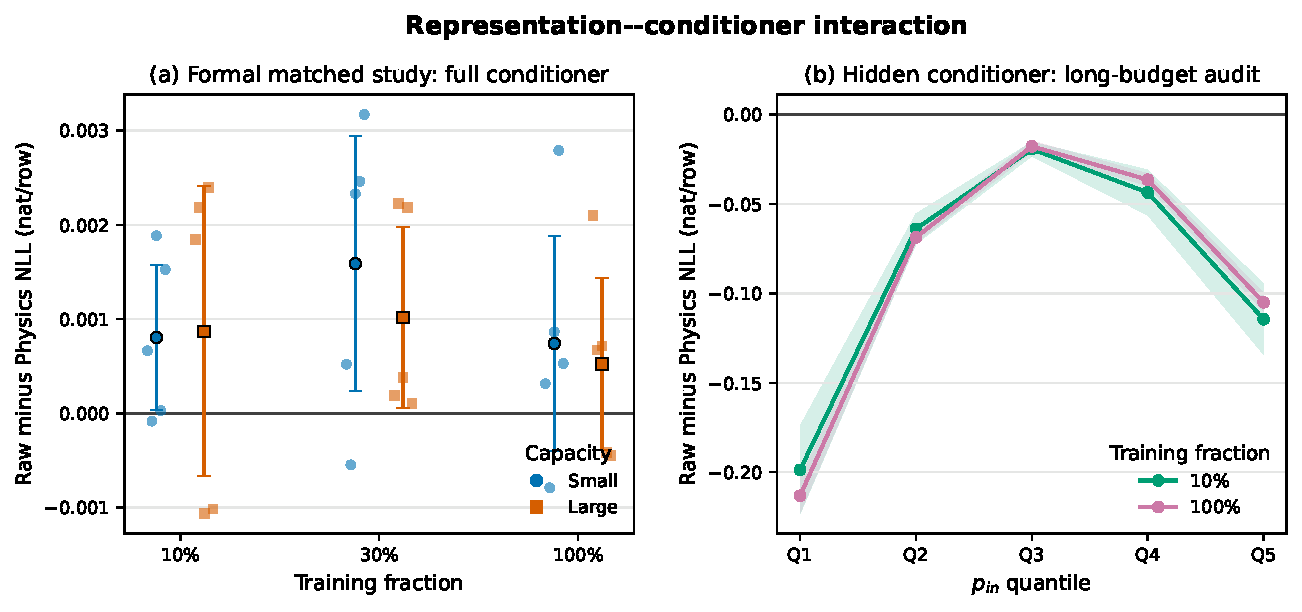
\includegraphics[width=0.92\linewidth]{figures/overview.pdf}
\caption{Historical paired Raw-minus-H contrasts. The original ``Physics'' label denotes H. The formal matrix is near zero and
 mixed, whereas the common-budget Hidden comparison is negative at both training
 fractions. Error bars and shaded bands are descriptive seed spread, not
 independence-based confidence intervals. Negative values favor Raw.}
\label{fig:interaction}
\end{figure}

\subsection{Historical residual-location diagnostic}

Let $V=\pin$ and let $W$ denote the physical conditions retained by the Hidden
conditioner. For a deterministic center,
\begin{equation}
 \operatorname{Var}(R\mid V,W)=\operatorname{Var}(Y\mid V,W).
\end{equation}
Consequently, a broader residual standard deviation after pooling over $V$ is
not evidence that the translation changed the intrinsic conditional variance.

The train-only conditional audit uses eight $\pin$ bins inside each of six
exact $(t,q)$ physical strata. Within narrow bins, Raw and H have nearly
equal spread and skewness. Define the weighted between-bin location variance
for representation $X$ in physical stratum $w$ as
\begin{equation}
 L_X(w)=\sum_k \pi_{wk}\left(\bar X_{wk}-\bar X_w\right)^2,
\end{equation}
where $\bar X_{wk}$ is the mean in momentum bin $k$ and $\pi_{wk}$ is its
training-sample fraction. The stratum-level excess $L_R(w)-L_Y(w)$ is positive
in all six physical strata. The correlation analysis instead uses the
unweighted per-bin squared-location difference
\begin{equation}
 D_{wk}=(\bar R_{wk}-\bar R_w)^2-(\bar Y_{wk}-\bar Y_w)^2.
\end{equation}
Across the 48 condition-bin groups, $D_{wk}$ has Pearson correlation $-0.641$
and Spearman correlation $-0.577$ with the paired Raw-minus-H NLL gap. These
are descriptive associations among dependent groups, not causal estimates or
significance tests.

\begin{figure}[!htbp]
\centering
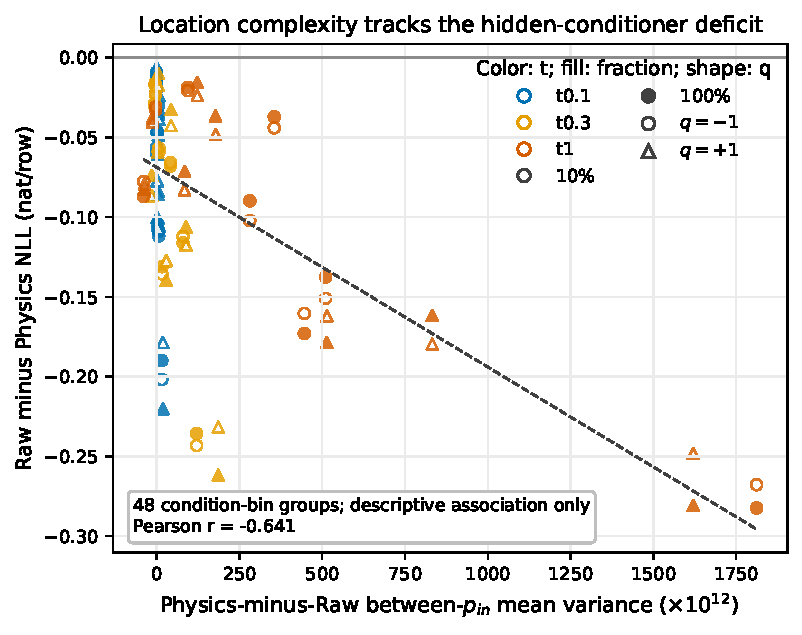
\includegraphics[width=0.92\linewidth]{figures/mechanism.pdf}
\caption{Historical location diagnostic. The original ``Physics'' label denotes H. H has larger between-$\pin$ residual-location
complexity in each physical stratum, and the groupwise complexity excess is
directionally associated with the NLL gap. The association is descriptive.}
\label{fig:mechanism}
\end{figure}

\subsection{Likelihood decomposition}

For the saved historical Hidden predictions, the audit recomputed Eq.~\eqref{eq:likelihood}
from the exported base log-density, Jacobian, and learned-flow $\log F_\theta(b)$
terms. Across all 20 audited checkpoints, the Raw--H support-normalization
gap is numerically zero. The 10\% total gap is $-0.0880018$ nats per event and
the corresponding base-density/Jacobian gap is $-0.0880018$; at 100\% the two
values are $-0.0882160$ and $-0.0882160$. Reconstruction errors are below
$2\times10^{-6}$ nats, consistent with float32 export rounding.

No support-term contribution was resolved at the exported precision for these
examined historical checkpoints. This is not evidence about the corrected
checkpoints. It does not prove that residual-location complexity is the unique causal
source of the deficit. The defensible statement is: \emph{residual-location
incompatibility is supported by diagnostic evidence; its causal contribution
to the likelihood deficit remains unestablished.}

\begin{figure}[!htbp]
\centering
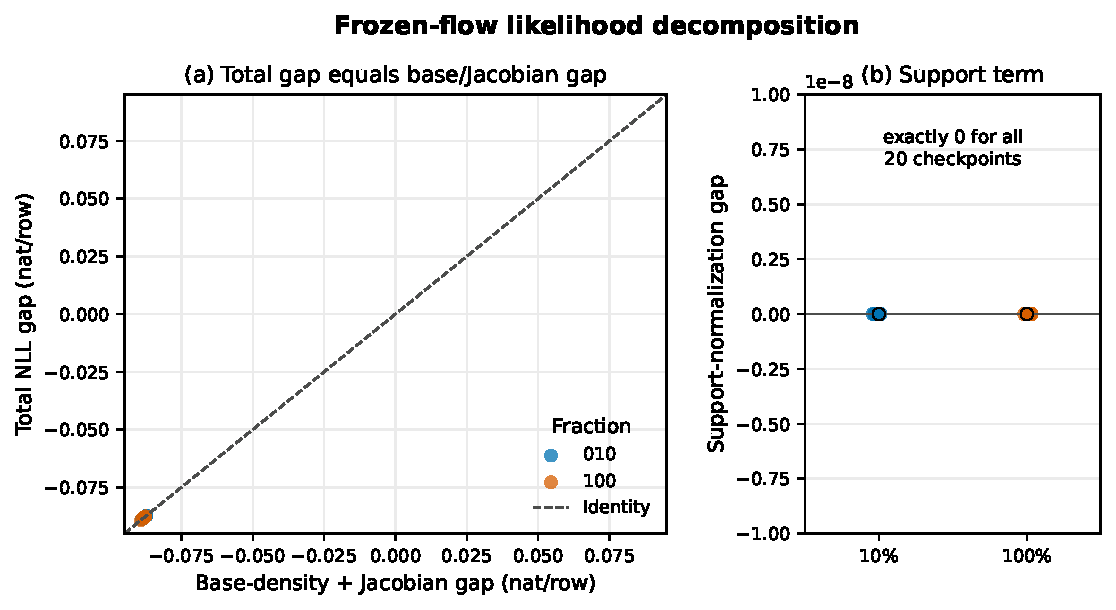
\includegraphics[width=0.92\linewidth]{figures/likelihood_decomposition.pdf}
\caption{Historical frozen-flow likelihood decomposition. The original ``Physics'' label denotes H. The observed Raw--H gap is
carried by the base-density/Jacobian term; the support-normalization difference
is zero to exported precision in the audited checkpoints.}
\label{fig:decomposition}
\end{figure}

\subsection{Historical frozen scoring}

The confirmation scorer evaluates existing checkpoints without refitting,
resplitting, or model selection. On block A, Full-conditioner contrasts are
$+0.001018$ and $+0.000615$ at 10\% and 100\%; Hidden contrasts are
$-0.088609$ and $-0.088773$. On block B, Full contrasts are $+0.000775$ and
$+0.000443$, while Hidden contrasts are $-0.087787$ and $-0.087957$.

The residual-location diagnostic transfers to all 12 block-by-stratum
combinations. This repeats the frozen erroneous-center score pattern; it is not
confirmation of newly trained CorrectedPhysics models or a causal mechanism. The
blocks were independent of representation-v2 development but had prior use in
the legacy W6/MDN workflow.

Table~\ref{tab:confirmation} retains the complete historical block means. The original historical scoring plot is preserved unchanged in the accompanying source archive.

\begin{table}[t]
\centering
\caption{Historical frozen scoring. Values are Raw minus H in
nats per event; negative values favor Raw.}
\label{tab:confirmation}
\begin{tabular}{llrr}
\toprule
Block & Conditioner & 10\% & 100\% \\
\midrule
A & Full & $+0.001018$ & $+0.000615$ \\
A & Hidden & $-0.088609$ & $-0.088773$ \\
B & Full & $+0.000775$ & $+0.000443$ \\
B & Hidden & $-0.087787$ & $-0.087957$ \\
\bottomrule
\end{tabular}
\end{table}


\clearpage
\end{document}
